

\documentclass[11pt,compress,t,notes=noshow]{beamer}

\usepackage[english]{babel}
\usepackage{dsfont}
\newcommand\bmmax{2}
\usepackage{bm}
\usepackage{bbm}
\usepackage{verbatim}
\usepackage{amsmath}
\usepackage{amsfonts}
\usepackage{csquotes}
\usepackage{multirow}
\usepackage{longtable}
\usepackage{enumerate}
\usepackage[absolute,overlay]{textpos}
\usepackage{psfrag}
\usepackage{algorithm}
\usepackage{algorithmicx}
\usepackage{algpseudocode}
\usepackage{eqnarray}
\usepackage{multimedia}
\usepackage{media9}
\usepackage{arydshln}
\usepackage{tabularx}
\usepackage{placeins}
\usepackage{tikz}
\usepackage{setspace}
\usepackage{wrapfig}
\usepackage{tcolorbox}
\usepackage[export]{adjustbox}
\usepackage{siunitx}
\usetikzlibrary{shapes,arrows,automata,positioning,calc}
\tikzset{
  %Define standard arrow tip
  >=stealth',
  %Define style for boxes
  punkt/.style={
    rectangle,
    rounded corners,
    draw=black, very thick,
    text width=6.5em,
    minimum height=2em,
    text centered},
  % Define arrow style
  pil/.style={
    ->,
    thick,
    shorten <=2pt,
    shorten >=2pt,}
}
\usepackage{subfig}

%new environments

\newenvironment{vbframe}  %frame with breaks and verbatim
{
 \begin{frame}[containsverbatim,allowframebreaks]
}
{
\end{frame}
}

\newenvironment{vframe}  %frame with verbatim without breaks (to avoid numbering one slided frames)
{
 \begin{frame}[containsverbatim]
}
{
\end{frame}
}

\newenvironment{blocki}[1]   % itemize block
{
 \begin{block}{#1}\begin{itemize}
}
{
\end{itemize}\end{block}
}

\newenvironment{fragileframe}[2]{  %fragile frame with framebreaks
\begin{frame}[allowframebreaks, fragile, environment = fragileframe]
\frametitle{#1}
#2}
{\end{frame}}


\newcommand{\myframe}[2]{  %short for frame with framebreaks
\begin{frame}[allowframebreaks]
\frametitle{#1}
#2
\end{frame}}

\newcommand{\remark}[1]{
  \textbf{Remark:} #1
}

%%%%%%%%%%%%%%%%%%%%%%%%%%%%%%%%%%%%%%%%%%%%%%%%%%%%%%%%%%%%%%%%%%%%%%%%%%%%%%%

% basic latex stuff
\newcommand{\pkg}[1]{{\fontseries{b}\selectfont #1}} %fontstyle for R packages
\newcommand{\lz}{\vspace{0.5cm}} %vertical space
\newcommand{\dlz}{\vspace{1cm}} %double vertical space
\newcommand{\oneliner}[1] % Oneliner for important statements
{\begin{block}{}\begin{center}\begin{Large}#1\end{Large}\end{center}\end{block}}


%\usetheme{lmu-lecture}
\usepackage{../style/lmu-lecture}

\let\code=\texttt
\let\proglang=\textsf

\setkeys{Gin}{width=0.9\textwidth}


\title{Deep Learning}
\author{Mina Rezaei}
\institute{Department of Statistics -- LMU Munich}
\date{Winter Semester 2021}

\setbeamertemplate{frametitle}{\expandafter\uppercase\expandafter\insertframetitle}

%\begin{document}
%\sloppy
%\end{document}


\input{../../latex-math/basic-math}
\input{../../latex-math/basic-ml}
\input{../../latex-math/ml-nn}

\begin{document}

\lecturechapter{1}{History of Neural Networks}
\lecture{Deep Learning}


%%%%%%%%%%%%%%%%%%%%%%%%%%%%%%%%%%%%%%%%%%%%%%%%%%%%%%%%%%%%%%%%%%

\begin{vbframe}{A brief history of neural networks}
  
  \begin{itemize}
    \item \pkg{1943:} The first artificial neuron, the "Threshold Logic Unit (TLU)", was proposed by Warren McCulloch \& Walter Pitts.
    \begin{itemize}
      \item In this model the neuron fires a $+1$ if the input exceeds a certain threshold $\phi$.
      \item However, this model did not have adjustable weights, so learning could only be achieved by changing the threshold $\phi$.
    \end{itemize}
    % Source: https://en.wikipedia.org/wiki/Artificial_neuron#History
  \end{itemize}
\framebreak
  \begin{itemize}
    \item \pkg{1957:} The perceptron was invented by Frank Rosenblatt. 
  \end{itemize}
    \begin{figure}
        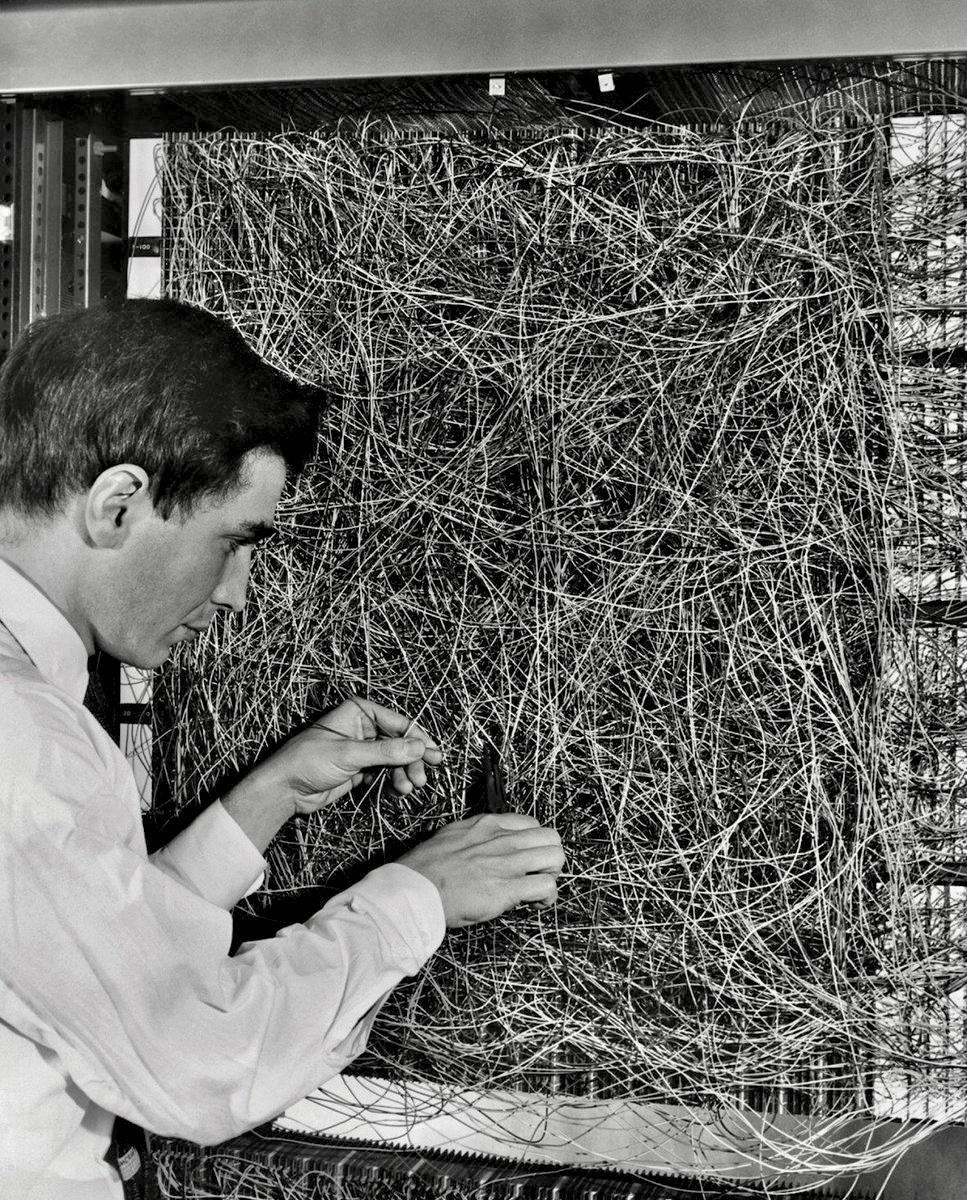
\includegraphics[width=4cm]{plots/Walter.jpg}
        \caption{Frank Rosenblatt with a Mark I Perceptron machine, the first implementation of the perceptron algorithm in 1960. (https://en.wikipedia.org/wiki/Perceptron)}
    \end{figure}
\framebreak
  \begin{itemize}
    \item \pkg{1960:} ADALINE by Bernard Widrow \& Tef Hodd.
    \begin{itemize}
      \item Weights are now adjusted according to the weighted sum of the inputs.
    \end{itemize}
    % Source: https://en.wikipedia.org/wiki/ADALINE
    \item \pkg{1965:} Group method of data handling (also known as polynomial neural networks) by Alexey Ivakhnenko. The first learning algorithm for supervised deep feedforward multilayer perceptrons.
    % Source: http://people.idsia.ch/~juergen/firstdeeplearner.html (J?rgen Schmidhubers website)
    %         https://en.wikipedia.org/wiki/Group_method_of_data_handling
    \item \pkg{1969:} The first \enquote{AI Winter} kicked in.
    \begin{itemize}
      \item Marvin Minsky \& Seymour Papert proved that a perceptron cannot solve the XOR-Problem (linear separability).
      \item Less funding $\Rightarrow$ Standstill in AI/DL research
      % Source: https://en.wikipedia.org/wiki/Perceptrons_(book)#The_XOR_affair
      %         https://en.wikipedia.org/wiki/AI_winter
    \end{itemize}
  \end{itemize}
\framebreak
  \begin{itemize}
    \item \pkg{1985:} Multi-layered perceptron with backpropagation by David Rumelhart, Geoffrey Hinton and Ronald Williams.
    % Source: https://en.wikipedia.org/wiki/Backpropagation#History
    % Results: This was when Rumelhart, Williams, and Hinton demonstrated back propagation in a neural network could provide "interesting" distribution representations. Philosophically, this discovery brought to light the question within cognitive psychology of whether human understanding relies on symbolic logic (computationalism) or distributed representations (connectionism). http://www.dataversity.net/brief-history-deep-learning/
    \begin{itemize}
      \item Method to efficiently compute derivatives of differentiable composite functions.
      \item Backpropagation was developed already in 1970 by Seppo Linnainmaa.
      % Source: https://en.wikipedia.org/wiki/Seppo_Linnainmaa
    \end{itemize}
    \item \pkg{1985:} The second \enquote{AI Winter} kicked in.
    \begin{itemize}
      \item Overly optimistic/exaggerated expectations concerning potential of AI/DL.
      \item Angering investors, the phrase \enquote{AI} even reached a pseudoscience status.
      \item Kernel machines and graphical models both achieved good results on many important tasks.
      \item Some of the fundamental mathematical difficulties in modeling long sequences were identified.
      % Source http://www.dataversity.net/brief-history-deep-learning/
    \end{itemize}
    \item \pkg{2006:} Age of deep neural networks began.
    \begin{itemize}
      \item Geoffrey Hinton showed that a deep belief network could be efficiently trained using a strategy called greedy layer-wise pretraining.
      \item This wave of neural networks research popularized the use of the term deep learning to emphasize that researchers were now able to train deeper neural networks than had been possible before.
      \item At this time, deep neural networks outperformed competing AI systems based on other machine learning technologies as well as hand-designed functionality.
    \end{itemize}
  %\end{itemize}
\framebreak
      \item  Why now and not earlier?
      \begin{itemize}
    \vspace{2mm}
    \item Significantly bigger datasets.
    \vspace{2mm}
    \item Better algorithms (optimization chapter).
      \begin{itemize}
        \item Vanishing gradient problem (ReLu).
      \end{itemize}
      \vspace{2mm}
    \item Better regularization (regularization chapter).
    \vspace{2mm}
    \item Unsupervised representation learning (autoencoder chapter).
    \vspace{2mm}
    \item More layers inevitably lead to a significant increase of parameters.
      \begin{itemize}
        \item Back then, processing power was simply not capable to handle such huge amounts of parameters. \\
        $\Rightarrow$ Nowadays, deep neural networks are trained on GPUs (graphic processing units), not on CPUs (central processing units).
        \item Investment by industries and universities.
        \item Deep learning tools make learning and applying deep learning easier.
      \end{itemize}
  \end{itemize}
\end{itemize}
\framebreak
    History of DL Tools
    \begin{itemize}
    \item 1960: Mark 1 Preceptron
    \item 2002: Torch
    \item 2007: CUDA
    \item 2008: Theano
    \item 2014: Caffe
    \item 2015: TensorFlow 0.1
    \item 2017: PyTorch 0.1
    \item 2017: MXNet
    \item 2017: Caffe 2.0
    \item 2019: TensorFlow 2.0
  \end{itemize}
  \framebreak
  \vspace{15mm}
  \begin{figure}
    \centering
      \scalebox{1.1}{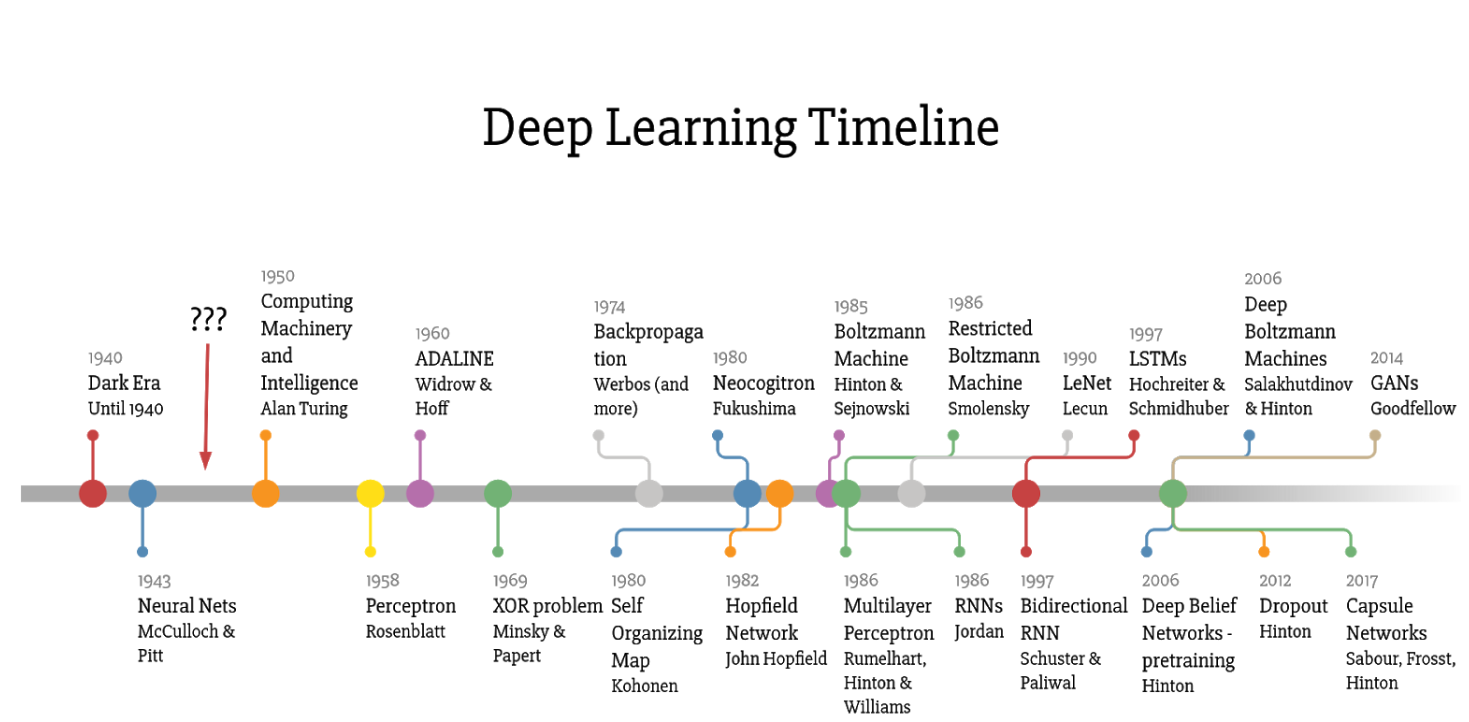
\includegraphics{plots/dl_timeline.png}}
      \caption{Credit: Favio Vazquez}
  \end{figure}
  \framebreak
 \begin{figure}
    \centering
    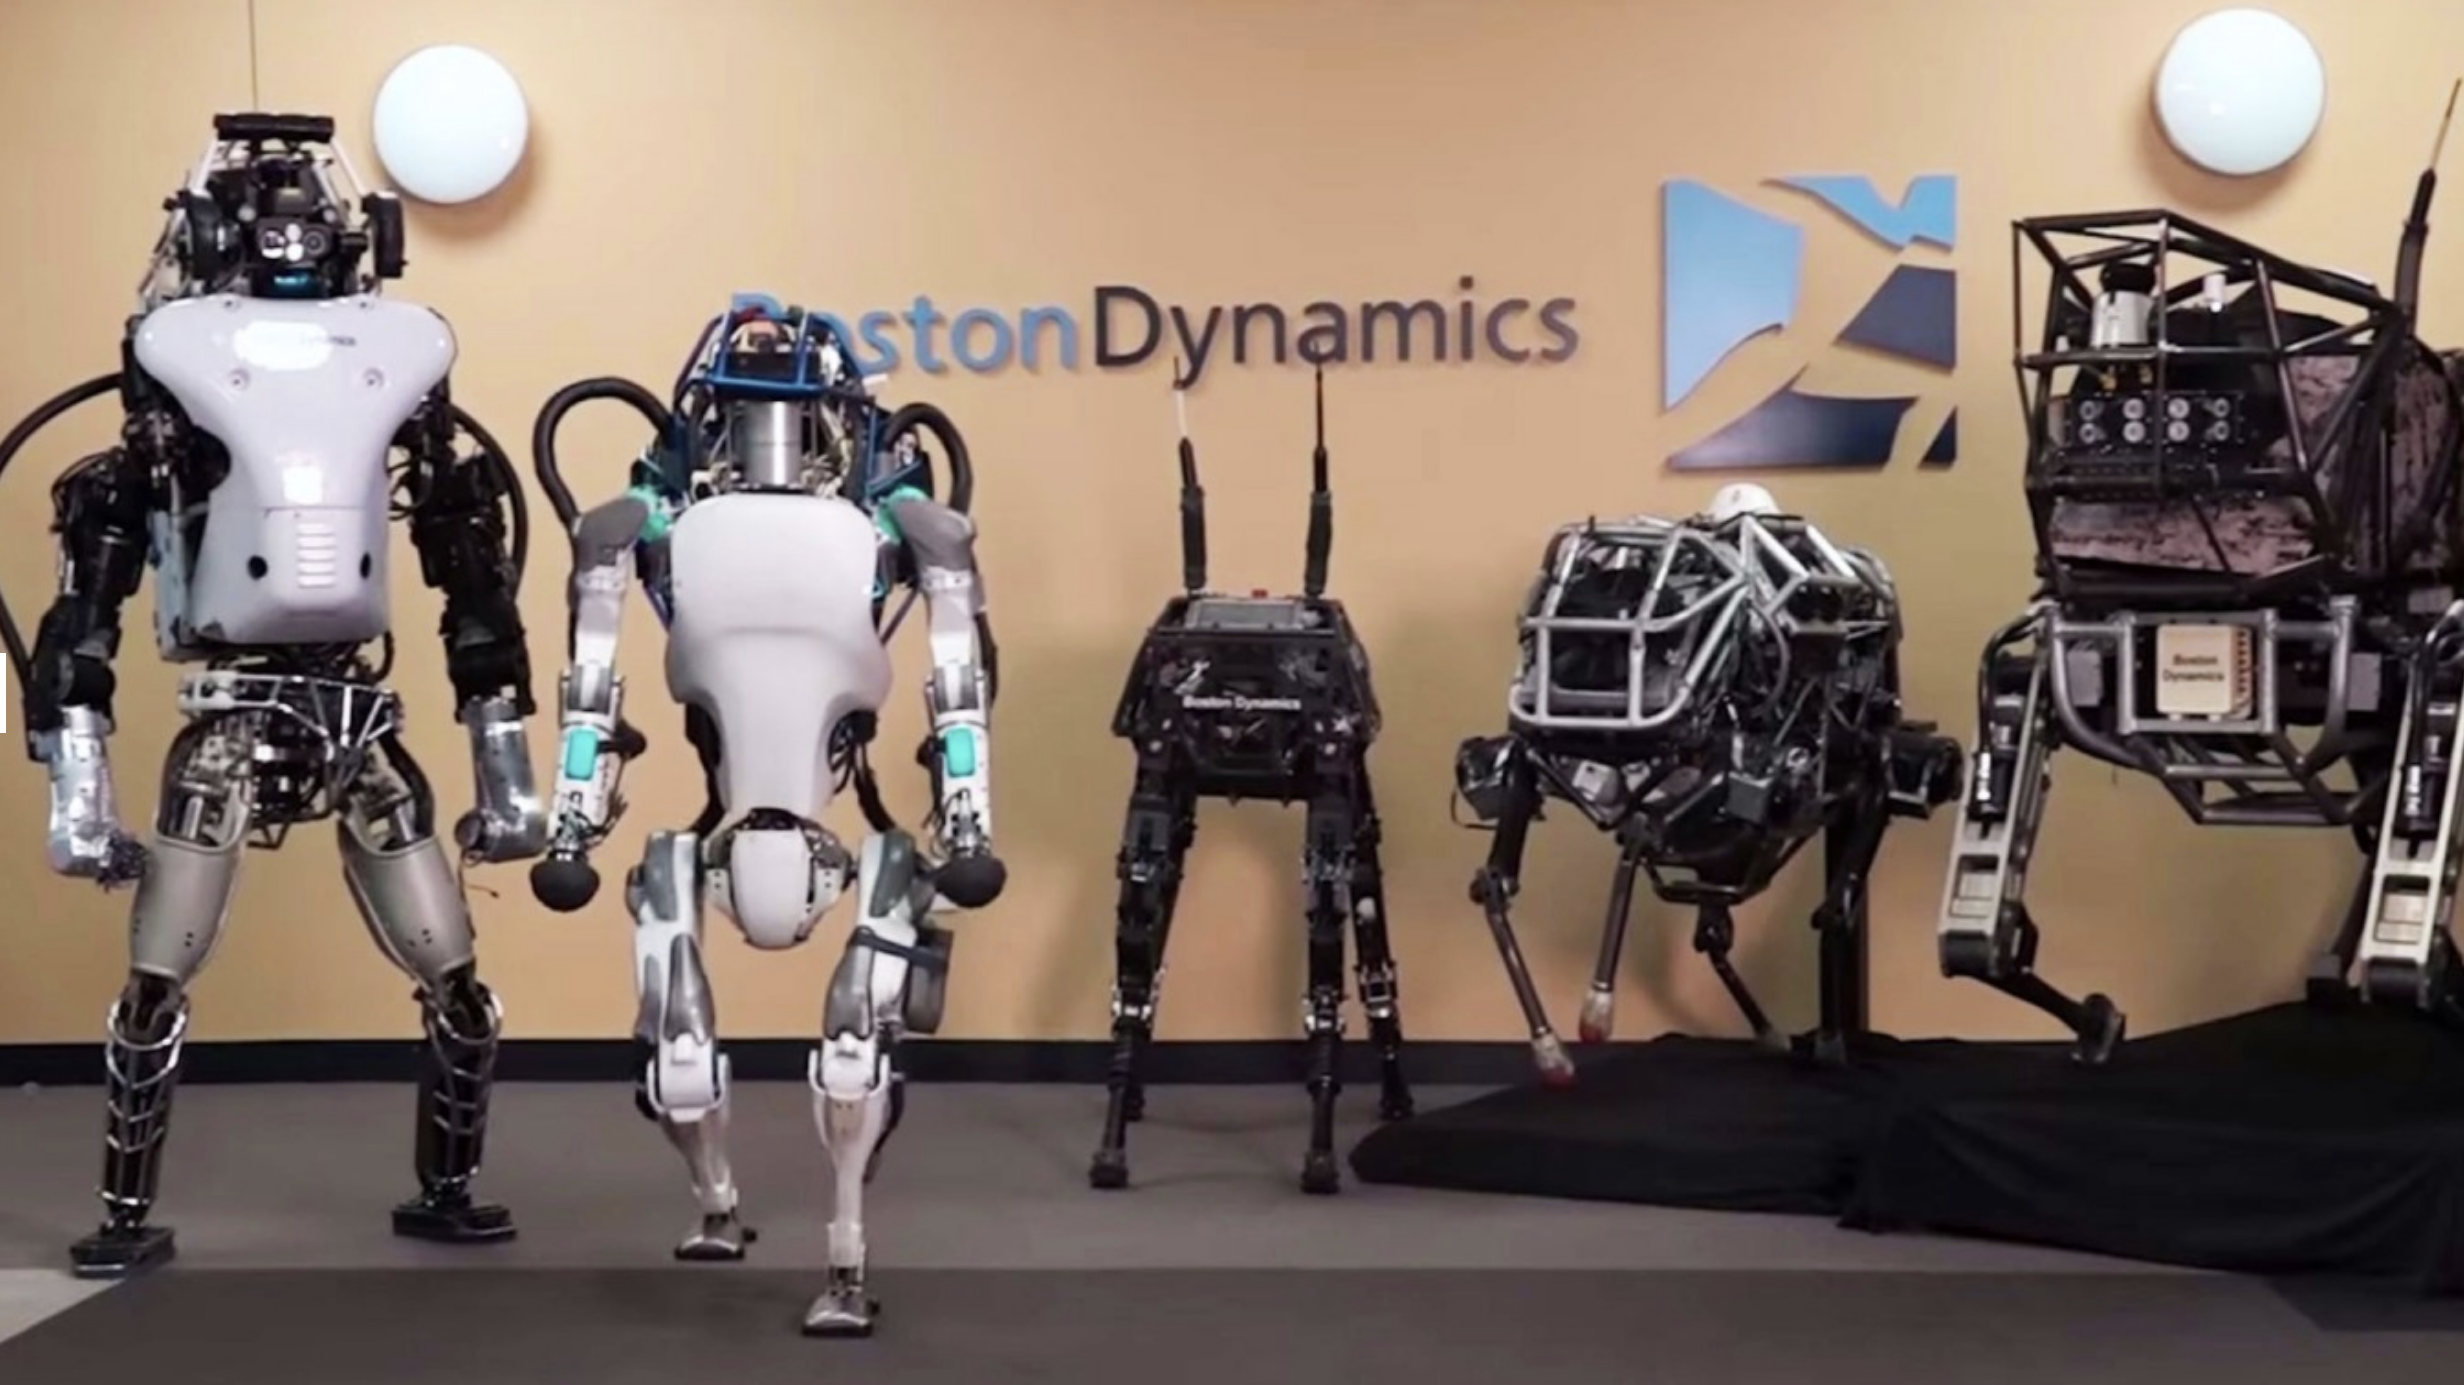
\includegraphics[width=10cm]{plots/bostondynamic.png}
    \caption{Boston Dynamic}
 \end{figure}
  \begin{figure}
    \centering
    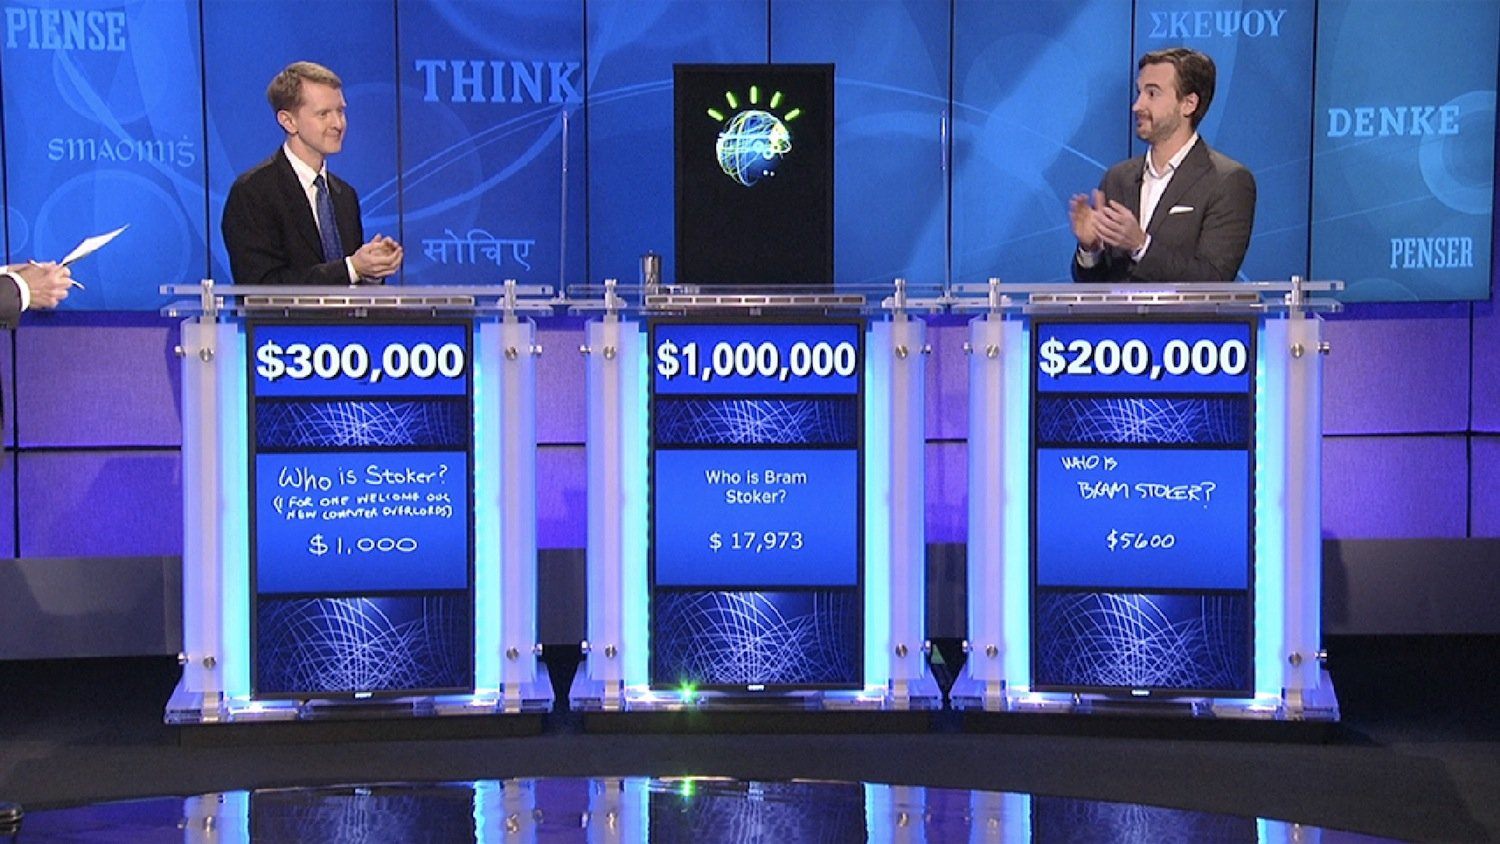
\includegraphics[width=10cm]{plots/ibmsupercomputer.jpg}
    \caption{IBM Supercomputer}
 \end{figure}
  \begin{figure}
    \centering
    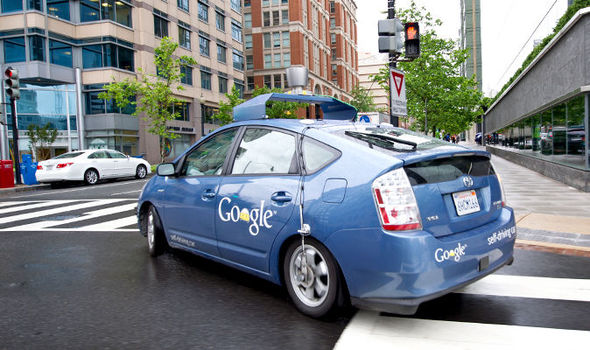
\includegraphics[width=10cm]{plots/selfdriving.jpg}
    \caption{Google Self driving car (Waymo)}
 \end{figure}
%\begin{figure}
%    \centering
%      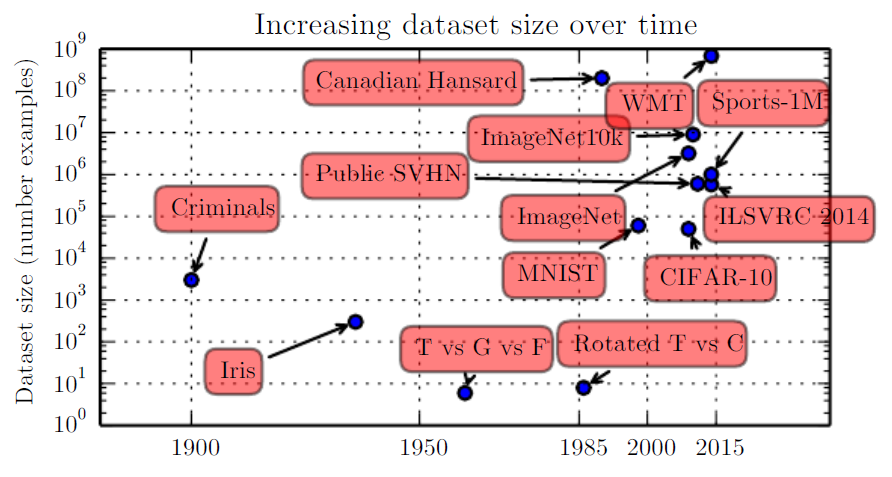
\includegraphics[width=10cm]{plots/dataset_size_over_time.png}
%      \caption{Dataset sizes over time (Goodfellow et al. (2016))}
%  \end{figure}
%\framebreak
%  \begin{figure}
%    \centering
%      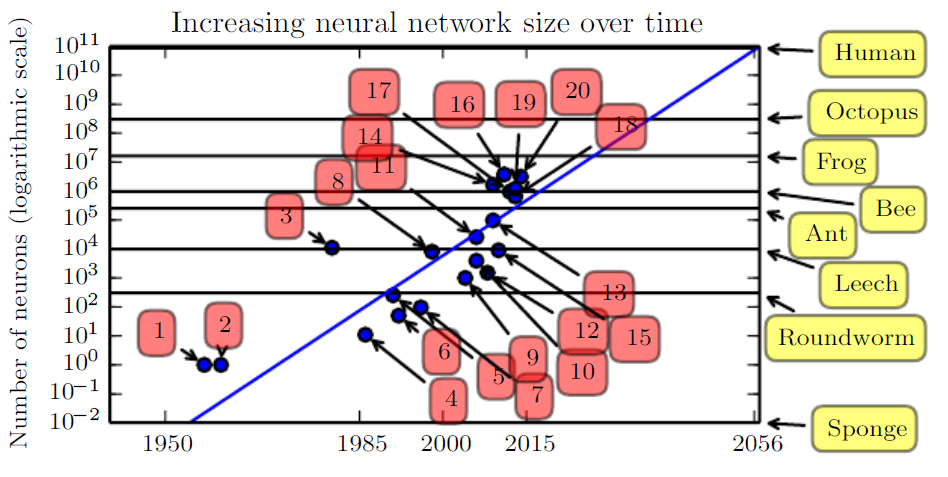
\includegraphics[width=10cm]{plots/network_size_over_time.png}
%      \caption{Network sizes over time. 1: Perceptron, 5: Recurrent neural network for speech recognition, 8: LeNet-5, 10: Deep belief network, 20: GoogLeNet. For more details, see: Goodfellow et al. (2016)}
%  \end{figure}
\end{vbframe}

\endlecture
\end{document}